% Options for packages loaded elsewhere
% \PassOptionsToPackage{unicode}{hyperref}
% \PassOptionsToPackage{hyphens}{url}
% \PassOptionsToPackage{dvipsnames,svgnames,x11names}{xcolor}
% %
% \documentclass[
%   11pt,
%   a4paperpaper,
% ]{article}

% \usepackage{amsmath,amssymb}
% \usepackage{iftex}
% \ifPDFTeX
%   \usepackage[T1]{fontenc}
%   \usepackage[utf8]{inputenc}
%   \usepackage{textcomp} % provide euro and other symbols
% \else % if luatex or xetex
%   \usepackage{unicode-math}
%   \defaultfontfeatures{Scale=MatchLowercase}
%   \defaultfontfeatures[\rmfamily]{Ligatures=TeX,Scale=1}
% \fi
% \usepackage{lmodern}
% \ifPDFTeX\else
%     % xetex/luatex font selection
% \fi
% % Use upquote if available, for straight quotes in verbatim environments
% \IfFileExists{upquote.sty}{\usepackage{upquote}}{}
% \IfFileExists{microtype.sty}{% use microtype if available
%   \usepackage[]{microtype}
%   \UseMicrotypeSet[protrusion]{basicmath} % disable protrusion for tt fonts
% }{}
% \makeatletter
% \@ifundefined{KOMAClassName}{% if non-KOMA class
%   \IfFileExists{parskip.sty}{%
%     \usepackage{parskip}
%   }{% else
%     \setlength{\parindent}{0pt}
%     \setlength{\parskip}{6pt plus 2pt minus 1pt}}
% }{% if KOMA class
%   \KOMAoptions{parskip=half}}
% \makeatother
% \usepackage{xcolor}
% \usepackage[lmargin=1in,rmargin=1in,tmargin=1in,bmargin=1in]{geometry}
% \setlength{\emergencystretch}{3em} % prevent overfull lines
% \setcounter{secnumdepth}{-\maxdimen} % remove section numbering
% % Make \paragraph and \subparagraph free-standing
% \ifx\paragraph\undefined\else
%   \let\oldparagraph\paragraph
%   \renewcommand{\paragraph}[1]{\oldparagraph{#1}\mbox{}}
% \fi
% \ifx\subparagraph\undefined\else
%   \let\oldsubparagraph\subparagraph
%   \renewcommand{\subparagraph}[1]{\oldsubparagraph{#1}\mbox{}}
% \fi


% \providecommand{\tightlist}{%
%   \setlength{\itemsep}{0pt}\setlength{\parskip}{0pt}}\usepackage{longtable,booktabs,array}
% \usepackage{calc} % for calculating minipage widths
% % Correct order of tables after \paragraph or \subparagraph
% \usepackage{etoolbox}
% \makeatletter
% \patchcmd\longtable{\par}{\if@noskipsec\mbox{}\fi\par}{}{}
% \makeatother
% % Allow footnotes in longtable head/foot
% \IfFileExists{footnotehyper.sty}{\usepackage{footnotehyper}}{\usepackage{footnote}}
% \makesavenoteenv{longtable}
% \usepackage{graphicx}
% \makeatletter
% \def\maxwidth{\ifdim\Gin@nat@width>\linewidth\linewidth\else\Gin@nat@width\fi}
% \def\maxheight{\ifdim\Gin@nat@height>\textheight\textheight\else\Gin@nat@height\fi}
% \makeatother
% % Scale images if necessary, so that they will not overflow the page
% % margins by default, and it is still possible to overwrite the defaults
% % using explicit options in \includegraphics[width, height, ...]{}
% \setkeys{Gin}{width=\maxwidth,height=\maxheight,keepaspectratio}
% % Set default figure placement to htbp
% \makeatletter
% \def\fps@figure{htbp}
% \makeatother

% \makeatletter
% \makeatother
% \makeatletter
% \makeatother
% \makeatletter
% \@ifpackageloaded{caption}{}{\usepackage{caption}}
% \AtBeginDocument{%
% \ifdefined\contentsname
%   \renewcommand*\contentsname{Table of contents}
% \else
%   \newcommand\contentsname{Table of contents}
% \fi
% \ifdefined\listfigurename
%   \renewcommand*\listfigurename{List of Figures}
% \else
%   \newcommand\listfigurename{List of Figures}
% \fi
% \ifdefined\listtablename
%   \renewcommand*\listtablename{List of Tables}
% \else
%   \newcommand\listtablename{List of Tables}
% \fi
% \ifdefined\figurename
%   \renewcommand*\figurename{Figure}
% \else
%   \newcommand\figurename{Figure}
% \fi
% \ifdefined\tablename
%   \renewcommand*\tablename{Table}
% \else
%   \newcommand\tablename{Table}
% \fi
% }
% \@ifpackageloaded{float}{}{\usepackage{float}}
% \floatstyle{ruled}
% \@ifundefined{c@chapter}{\newfloat{codelisting}{h}{lop}}{\newfloat{codelisting}{h}{lop}[chapter]}
% \floatname{codelisting}{Listing}
% \newcommand*\listoflistings{\listof{codelisting}{List of Listings}}
% \makeatother
% \makeatletter
% \@ifpackageloaded{caption}{}{\usepackage{caption}}
% \@ifpackageloaded{subcaption}{}{\usepackage{subcaption}}
% \makeatother
% \makeatletter
% \makeatother
% \ifLuaTeX
%   \usepackage{selnolig}  % disable illegal ligatures
% \fi
% \IfFileExists{bookmark.sty}{\usepackage{bookmark}}{\usepackage{hyperref}}
% \IfFileExists{xurl.sty}{\usepackage{xurl}}{} % add URL line breaks if available
% \urlstyle{same} % disable monospaced font for URLs
% \hypersetup{
%   pdftitle={Erasure statistics},
%   colorlinks=true,
%   linkcolor={blue},
%   filecolor={Maroon},
%   citecolor={Blue},
%   urlcolor={Blue},
%   pdfcreator={LaTeX via pandoc}}

% \title{Erasure statistics}
% \author{}
% \date{}

% \begin{document}
% \maketitle
\chapter{Erasure statistics}
\label{sec:appendix-erasure}

% \hypertarget{the-number-of-parities-required}{%
% \subsection{The number of parities
% required}

Let there be \(m\) original chunks and \(k\) parity chunks, such that
any \(m\) chunks out of the total \(n = m + k\) ones are fully
recoverable after the loss of any \(k\) of them. In the process of
retrieving the \(n\) chunks, what is the likelihood of overall data
corruption, given a per-chunk probability of error \(\epsilon\)?

By ``overall data corruption'', we mean that more than \(k\) chunks are
damaged in the data retrieval process. We assume that each chunk's
probability of error is both equal to and independent of other chunks. In that case, the
problem boils down to the independent drawing of \(n\) chunks, each of
which undergo a Bernoulli trial of being faulty with probability
\(\epsilon\). The total number of faulty chunks out of \(n\) independent
Bernoulli trials is given by the binomial distribution:
\begin{equation}\protect\hypertarget{eq-PMF-binomial}{}{
B(i, n, \epsilon)
= \binom{n}{i} \epsilon^k (1-\epsilon)^{n-i} .
}\label{eq:PMF-binomial}\end{equation} This expression is the
probability mass function for the binomial distribution, yielding the
probability that out of \(n\) chunks, exactly \(i\) will be
faulty---assuming that the per-chunk probability of error is
\(\epsilon\).

Since there are \(k\) parities out of the \(n\) chunks, the system can
tolerate up to \(k\) chunk errors. The probability that no more than
\(k\) errors accumulate can be expressed by summing
Equation~\ref{eq:PMF-binomial} over \(i\) up to \(k\):
\begin{equation}\protect\hypertarget{eq-CDF-binomial}{}{
P(k, n, \epsilon)
= \sum_{i=0}^k \binom{n}{i} \epsilon^k (1-\epsilon)^{n-i} ,
}\label{eq:CDF-binomial}\end{equation} which is the cumulative
distribution function of the binomial distribution.

The question we often want to answer is the following: given the number
of chunks \(n\) and a security constant \(\alpha\) such that that we want the
overall probability of data corruption to be below this value, how many
out of the \(n\) chunks should be parities? That is, in
Equation~\ref{eq:CDF-binomial} we are looking for the value of \(k\)
which will make \(P(k, n, \epsilon) = 1 - \alpha\)
(Figure~\ref{fig:alpha}). This can be obtained by inverting the
cumulative distribution function in \(k\), resulting in the quantile
function \(Q(1 - \alpha, n, \epsilon)\). While this inverse has no
convenient closed-form expression, it can be efficiently evaluated
numerically for any set of input parameters.

\begin{figure}[!ht]

{\centering 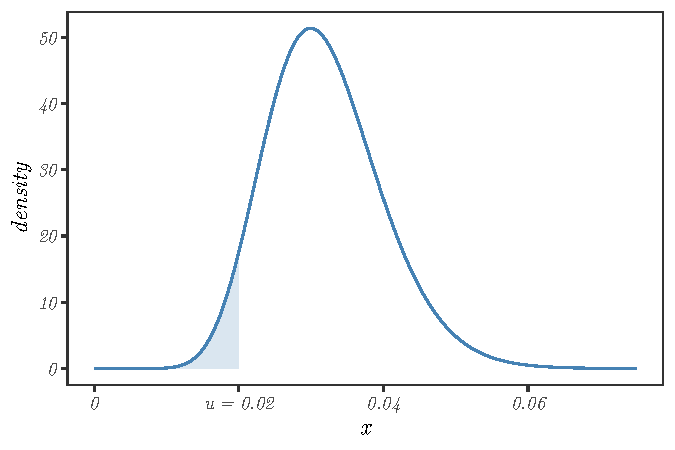
\includegraphics{fig/erasure/fig-alpha-1.pdf}

}

\caption{\label{fig:alpha}The point at \(k=17\) along the binomial
distribution, where the probability of exceeding this many errors
becomes less than \(\alpha = 10\%\). Here the total number of chunks is
\(n = 128\), and the per-chunk error rate is \(\epsilon = 0.1\).}

\end{figure}
Figures \ref{fig:perr-lin}-\ref{fig:maintain} summarize various aspects
of the required parities and error rates.

\begin{figure}[!ht]

{\centering \includegraphics{fig/erasure/fig-perr-lin-1.pdf}

}

\caption{\label{fig:perr-lin}The number of parities needed (ordinate) as
a function of the per-chunk error rate \(\epsilon\) (abscissa), for
keeping the probability of overall data corruption below given limits
(colors).}

\end{figure}

\begin{figure}[!ht]

{\centering \includegraphics{fig/erasure/fig-integrity-1.pdf}

}

\caption{\label{fig:integrity}The number of parities required (ordinate)
to keep the probability of overall data corruption at a given level
(abscissa), for various values of the per-chunk error rate \(\epsilon\)
(colours) and for \(n = 64\) chunks (left panel) and \(n = 128\) chunks
(right panel).}

\end{figure}

\begin{figure}[!ht]

{\centering \includegraphics{fig/erasure/fig-maintain-1.pdf}

}

\caption{\label{fig:maintain}Number of chunks (abscissa) and the
corresponding required number of parities (ordinate) such that will
maintain the same overall probability of no data corruption as would be
the case with 128 chunks, an original number of parities indicated by
the colors, and a likelihood \(\epsilon\) of an erroneous retrieval of a
single chunk indicated in the panel headers. (These probabilities are
listed in Table~\ref{tbl:baseline-param}.)}

\end{figure}

Table~\ref{tbl:baseline-param} summarizes the number of chunks that are
maintainable for a given number of parities \(k\) and per-chunk error
rate \(\epsilon\) such that the odds of data corruption
stays below 1 in a million, i.e., \(\alpha = 10^{-6}\). The first column of this table is the
number of parities, followed by various per-chunk error rates. The
entries in those subsequent columns are the number of chunks.

\hypertarget{tbl:baseline-param}{}
\begin{longtable}[]{@{}
  >{\raggedleft\arraybackslash}p{(\columnwidth - 8\tabcolsep) * \real{0.1268}}
  >{\raggedleft\arraybackslash}p{(\columnwidth - 8\tabcolsep) * \real{0.2113}}
  >{\raggedleft\arraybackslash}p{(\columnwidth - 8\tabcolsep) * \real{0.2113}}
  >{\raggedleft\arraybackslash}p{(\columnwidth - 8\tabcolsep) * \real{0.2254}}
  >{\raggedleft\arraybackslash}p{(\columnwidth - 8\tabcolsep) * \real{0.2254}}@{}}
\caption{\label{tbl:baseline-param}For a given number of parities (first
column) and per-chunk error rate (subsequent columns), how many chunks
can be supported to still have an overall data corruption probability
less than \(\alpha = 10^{-6}\)? The number of chunks is the raw number,
without the supporting parities.}\tabularnewline
\toprule\noalign{}
% \begin{minipage}[b]{\linewidth}\raggedleft
% parities
% \end{minipage} & \begin{minipage}[b]{\linewidth}\raggedleft
% error rate: 1\%
% \end{minipage} & \begin{minipage}[b]{\linewidth}\raggedleft
% error rate: 5\%
% \end{minipage} & \begin{minipage}[b]{\linewidth}\raggedleft
% error rate: 10\%
% \end{minipage} & \begin{minipage}[b]{\linewidth}\raggedleft
% error rate: 50\%
% \end{minipage} \\

% \midrule\noalign{}
% \endfirsthead
% \toprule\noalign{}
% \begin{minipage}[b]{\linewidth}\raggedleft
% parities
% \end{minipage} & \begin{minipage}[b]{\linewidth}\raggedleft
% error rate: 1\%
% \end{minipage} & \begin{minipage}[b]{\linewidth}\raggedleft
% error rate: 5\%
% \end{minipage} & \begin{minipage}[b]{\linewidth}\raggedleft
% error rate: 10\%
% \end{minipage} & \begin{minipage}[b]{\linewidth}\raggedleft
% error rate: 50\%
% \end{minipage} \\
% \midrule\noalign{}
% \endhead
% \bottomrule\noalign{}
% \endlastfoot
& \multicolumn{4}{c}{uniform and independent error rate of chunk retrieval}\\
parities& 1\%&5\%&10\%&50\%\\
\toprule
1 & & & & \\
2 & & & & \\
3 & 1 & & & \\
4 & 5 & & & \\
5 & 14 & 1 & & \\
6 & 28 & 3 & 1 & \\
7 & 46 & 6 & 2 & \\
8 & 68 & 10 & 3 & \\
9 & 94 & 15 & 5 & \\
10 & & 20 & 8 & \\
11 & & 26 & 10 & \\
12 & & 32 & 13 & \\
13 & & 39 & 16 & \\
14 & & 46 & 19 & \\
15 & & 53 & 22 & \\
16 & & 61 & 26 & \\
17 & & 69 & 29 & \\
18 & & 77 & 33 & \\
19 & & 86 & 37 & \\
20 & & 95 & 41 & 1 \\
21 & & 104 & 45 & 1 \\
22 & & & 50 & 1 \\
23 & & & 54 & 1 \\
24 & & & 59 & 2 \\
25 & & & 63 & 2 \\
26 & & & 68 & 2 \\
27 & & & 73 & 3 \\
28 & & & 77 & 3 \\
29 & & & 82 & 3 \\
30 & & & 87 & 4 \\
31 & & & 92 & 4 \\
32 & & & & 5 \\
33 & & & & 5 \\
34 & & & & 5 \\
35 & & & & 6 \\
36 & & & & 6 \\
37 & & & & 7 \\
38 & & & & 7 \\
39 & & & & 8 \\
40 & & & & 8 \\
41 & & & & 9 \\
42 & & & & 9 \\
43 & & & & 9 \\
44 & & & & 10 \\
45 & & & & 10 \\
46 & & & & 11 \\
47 & & & & 11 \\
48 & & & & 12 \\
49 & & & & 13 \\
50 & & & & 13 \\
51 & & & & 14 \\
52 & & & & 14 \\
53 & & & & 15 \\
54 & & & & 15 \\
55 & & & & 16 \\
56 & & & & 16 \\
57 & & & & 17 \\
58 & & & & 17 \\
59 & & & & 18 \\
60 & & & & 19 \\
61 & & & & 19 \\
62 & & & & 20 \\
63 & & & & 20 \\
64 & & & & 21 \\
65 & & & & 21 \\
66 & & & & 22 \\
67 & & & & 23 \\
68 & & & & 23 \\
69 & & & & 24 \\
70 & & & & 24 \\
71 & & & & 25 \\
72 & & & & 26 \\
73 & & & & 26 \\
74 & & & & 27 \\
75 & & & & 27 \\
76 & & & & 28 \\
77 & & & & 29 \\
78 & & & & 29 \\
79 & & & & 30 \\
80 & & & & 30 \\
81 & & & & 31 \\
82 & & & & 32 \\
83 & & & & 32 \\
84 & & & & 33 \\
85 & & & & 34 \\
86 & & & & 34 \\
87 & & & & 35 \\
88 & & & & 36 \\
89 & & & & 36 \\
90 & & & & 37 \\
91 & & & & 37 \\
\end{longtable}

Table~\ref{tbl:baseline-param-encrypted} is structured similarly, but
for encrypted chunks. Each encrypted chunk takes up 2 slots, but the
parity chunks still only use a single one. Thus, the number of effective
chunk slots used is obtained as twice the number of chunks plus the
number of parities.

\hypertarget{tbl:baseline-param-encrypted}{}
\begin{longtable}[]{@{}
  >{\raggedleft\arraybackslash}p{(\columnwidth - 8\tabcolsep) * \real{0.1268}}
  >{\raggedleft\arraybackslash}p{(\columnwidth - 8\tabcolsep) * \real{0.2113}}
  >{\raggedleft\arraybackslash}p{(\columnwidth - 8\tabcolsep) * \real{0.2113}}
  >{\raggedleft\arraybackslash}p{(\columnwidth - 8\tabcolsep) * \real{0.2254}}
  >{\raggedleft\arraybackslash}p{(\columnwidth - 8\tabcolsep) * \real{0.2254}}@{}}
\caption{\label{tbl:baseline-param-encrypted}As
Table~\ref{tbl:baseline-param}, but for encrypted chunks. The maximum
number of encrypted chunks is 64, so each encrypted chunks reference is a double segment (a hash reference, plus the segment-sized decryption key.  The parity chunks on the other hand and parities extended the encrypted chunks, so they themselves do not need to b encrypted, so their reference is a single segment long
Consequently, the number of effective chunk slots used is obtained as
twice the number of chunks in any one of columns 2-5, plus the number of
parities in column 1.}\tabularnewline
% \toprule\noalign{}
% \begin{minipage}[b]{\linewidth}\raggedleft
% parities
% \end{minipage} & \begin{minipage}[b]{\linewidth}\raggedleft
% error rate: 1\%
% \end{minipage} & \begin{minipage}[b]{\linewidth}\raggedleft
% error rate: 5\%
% \end{minipage} & \begin{minipage}[b]{\linewidth}\raggedleft
% error rate: 10\%
% \end{minipage} & \begin{minipage}[b]{\linewidth}\raggedleft
% error rate: 50\%
% \end{minipage} \\
% \midrule\noalign{}
% \endfirsthead
% \toprule\noalign{}
% \begin{minipage}[b]{\linewidth}\raggedleft
% parities
% \end{minipage} & \begin{minipage}[b]{\linewidth}\raggedleft
% error rate: 1\%
% \end{minipage} & \begin{minipage}[b]{\linewidth}\raggedleft
% error rate: 5\%
% \end{minipage} & \begin{minipage}[b]{\linewidth}\raggedleft
% error rate: 10\%
% \end{minipage} & \begin{minipage}[b]{\linewidth}\raggedleft
% error rate: 50\%
% \end{minipage} \\
% \midrule\noalign{}
% \endhead
% \bottomrule\noalign{}
% \endlastfoot
& \multicolumn{4}{c}{uniform and independent error rate of chunk retrieval}\\
parities& 1\%&5\%&10\%&50\%\\
\toprule
4 & 2 & & & \\
5 & 7 & & & \\
6 & 14 & 1 & & \\
7 & 23 & 3 & 1 & \\
8 & 34 & 5 & 1 & \\
9 & 47 & 7 & 2 & \\
10 & & 10 & 4 & \\
11 & & 13 & 5 & \\
12 & & 16 & 6 & \\
13 & & 19 & 8 & \\
14 & & 23 & 9 & \\
15 & & 26 & 11 & \\
16 & & 30 & 13 & \\
17 & & 34 & 14 & \\
18 & & 38 & 16 & \\
19 & & 43 & 18 & \\
20 & & 47 & 20 & \\
21 & & 52 & 22 & \\
22 & & & 25 & \\
23 & & & 27 & \\
24 & & & 29 & 1 \\
25 & & & 31 & 1 \\
26 & & & 34 & 1 \\
27 & & & 36 & 1 \\
28 & & & 38 & 1 \\
29 & & & 41 & 1 \\
30 & & & 43 & 2 \\
31 & & & 46 & 2 \\
32 & & & & 2 \\
33 & & & & 2 \\
34 & & & & 2 \\
35 & & & & 3 \\
36 & & & & 3 \\
37 & & & & 3 \\
38 & & & & 3 \\
39 & & & & 4 \\
40 & & & & 4 \\
41 & & & & 4 \\
42 & & & & 4 \\
43 & & & & 4 \\
44 & & & & 5 \\
45 & & & & 5 \\
46 & & & & 5 \\
47 & & & & 5 \\
48 & & & & 6 \\
49 & & & & 6 \\
50 & & & & 6 \\
51 & & & & 7 \\
52 & & & & 7 \\
53 & & & & 7 \\
54 & & & & 7 \\
55 & & & & 8 \\
56 & & & & 8 \\
57 & & & & 8 \\
58 & & & & 8 \\
59 & & & & 9 \\
60 & & & & 9 \\
61 & & & & 9 \\
62 & & & & 10 \\
63 & & & & 10 \\
64 & & & & 10 \\
65 & & & & 10 \\
66 & & & & 11 \\
67 & & & & 11 \\
68 & & & & 11 \\
69 & & & & 12 \\
70 & & & & 12 \\
71 & & & & 12 \\
72 & & & & 13 \\
73 & & & & 13 \\
74 & & & & 13 \\
75 & & & & 13 \\
76 & & & & 14 \\
77 & & & & 14 \\
78 & & & & 14 \\
79 & & & & 15 \\
80 & & & & 15 \\
81 & & & & 15 \\
82 & & & & 16 \\
83 & & & & 16 \\
84 & & & & 16 \\
85 & & & & 17 \\
86 & & & & 17 \\
87 & & & & 17 \\
88 & & & & 18 \\
89 & & & & 18 \\
90 & & & & 18 \\
91 & & & & 18 \\
\end{longtable}

% \hypertarget{the-special-case-of-a-single-chunk}{%
% \subsection{The special case of a single
% chunk}
% \label{sec:the-special-case-of-a-single-chunk}}

Finally, an important special case is the required number of parities
for just a single chunk (in which case the ``parities'' may as well be
thought of as simple duplicates) to squeeze the probability of data
corruption below a certain level \(\alpha\). For this special case, an
explicit formula can be given. If the probability of one of these
parities being faulty is \(\epsilon\), then assuming independence, the
probability that \(n\) parities are faulty is \(\epsilon^n\). Here we
can write \(n = k + 1\); that is, we have one ``original'' chunk and the
rest of them are the \(k\) parities. Keeping the overall error
probability below \(\alpha\) then means that
\begin{equation}\protect\hypertarget{eq:onechunk}{}{
\epsilon^{k+1}
= \alpha
}\label{eq:onechunk}\end{equation} must be satisfied. Taking logarithms
on both sides and rearranging, we get
\begin{equation}\protect\hypertarget{eq-onechunk-parities}{}{
k
= \frac{\log(\alpha)}{\log(\epsilon)} - 1 .
}\label{eq:onechunk-parities}\end{equation} This is the number of
replicas that a chunk without sisters (and without parent context) is required to have to keep the overall data
corruption probability below \(\alpha\).

The base of the log in Equation~\ref{eq:onechunk-parities} is arbitrary.
This means that if we use base-10 logarithms and assume that
\(\alpha = 10^{-6}\), we get the simpler
\begin{equation}\protect\hypertarget{eq:onechunk-special}{}{
k
= \frac{6}{|\log_{10}(\epsilon)|} - 1 .
}\label{eq-onechunk-special}\end{equation} For example, if the per-chunk
error rate is ten percent (\(\epsilon = 0.1\)), then
\(|\log_{10}(\epsilon)| = |\log_{10}(1/10)| = 1\), and so
\(k = 6/1 - 1 = 5\) replicas are needed. If instead the per-chunk error
rate is just one percent (\(\epsilon = 0.01\)), then only
\(k = 6/2 - 1 = 2\) parities are necessary. Overall, for the same per-chunk error rates as in
Table~\ref{tbl:baseline-param}, we get:

\hypertarget{tbl:single-chunk}{}
\begin{longtable}[]{@{}lr@{}}
\caption{\label{tbl:single-chunk}For a given per-chunk error rate (first
column), how many replicas (second column) are required of a single
chunk to keep the overall data corruption probability below
\(\alpha = 10^{-6}\)?}\tabularnewline
\toprule\noalign{}
error rate & parities required \\
\midrule\noalign{}
\endfirsthead
\toprule\noalign{}
error rate & parities required \\
\midrule\noalign{}
\endhead
\bottomrule\noalign{}
\endlastfoot
1\% & 2 \\
5\% & 4 \\
10\% & 5 \\
50\% & 19 \\
\end{longtable}



% \end{document}
